\documentclass{report}
\usepackage[utf8]{inputenc}
\setlength{\parindent}{0em}
\setlength{\parskip}{1em}
\usepackage[svgnames]{xcolor}
\usepackage{listings}
\usepackage{pdfpages}

%\definecolor{termcolor}{RGB}{1.0, 0.97, 0.86}
%\definecolor{listingcolor}{RGB}{0.61, 0.87, 1.0}

\lstdefinestyle{termstyle}{
frame=single,
backgroundcolor=\color{Cornsilk},   
basicstyle=\verbatim@font\small,
numbers=none,
tabsize=2
}

\lstdefinestyle{listingstyle}{
frame=single,
backgroundcolor=\color{LightSkyBlue},   
basicstyle=\verbatim@font\small,
numbers=left,
numberstyle=\tiny,                    
tabsize=2
}



\title{MSc Scientific Computing Dissertation\\ARM Cluster Benchmarks}
\author{John Duffy}
\date{September 2020}

\begin{document}

\maketitle

\tableofcontents


%
% PART I
%
\part{Project Report}


%
% CHAPTER 
%
\chapter{Introduction}


%
% CHAPTER
%
\chapter{ARM Architectures for HP}


%
% CHAPTER
%
\chapter{The Aerin Cluster}



%
% PART II
%
\part{Benchmarks}


%
% CHAPTER
%
\chapter{High Performance Linpack (HPL) Benchmark}

\section{Introduction}



%
% CHAPTER
%
\chapter{HPC Challenge (HPCC) Benchmark}

\section{Introduction}


%
% CHAPTER
%
\chapter{High Performance Conjugate Gradients (HPCG) Benchmark}

\section{Introduction}



\section{Introduction}

\begin{verbatim}
https://github.com/johnduffymsc/picluster
\end{verbatim}


\subsection{Aims}

\subsubsection{Investigate Maximum Achievable Linpack Performance}

Efficiency... achieved vs theoretical maximum


\subsubsection{Investigate Gflops/Watt}

Green500 ranking...


\subsubsection{Overview of Competitive Available Gflops/£}

Buy lots of Pi's, or buy a bigger machine...

Plot Gflops vs £...


\subsection{Typography}

This is a computer name...

\verb|node1|

This is a command to type...

\lstset{style=termstyle}
\begin{lstlisting}[]
$ cat /proc/softirqs
\end{lstlisting}

And this is the command output...

\lstset{style=termstyle}
\begin{lstlisting}
                    CPU0       CPU1       CPU2       CPU3       
          HI:          1          0          0          1
       TIMER:    3835342    3454143    3431155    3431023
      NET_TX:      36635          0          0          0
      NET_RX:     509189        146        105        121
       BLOCK:      95326       4367       4311       4256
    IRQ_POLL:          0          0          0          0
     TASKLET:       4900          3          4         25
       SCHED:     444569     267214     218701     189120
     HRTIMER:         67          0          0          0
         RCU:     604466     281455     260784     277699
\end{lstlisting}

% TODO: Change to Ubuntu /etc/hosts...
This is a file listing...

\lstset{style=listingstyle}
\lstinputlisting[caption=/etc/hosts]{/etc/hosts}



\section{Raspberry Pi 4 Model B}

\subsection{Description}

Photo...

Description...

Highlights...

Limitations...

Reference data sheet in Appendix...



\subsection{Theoretical Maximum Performance (Gflop/s)}

The Raspberry Pi 4 Model B uses the Broadcom BCM2711 System on a Chip (Soc).

Block diagram from Cortex-A72 Software Optimisation Guide

4 cores

1.5 GHz

128 bit SIMD

4 GB memory (our chosen model)

Caches...

Pipeline...

Simplistically, ...

This ignores instructions pipelining benefits...



\section{Pi Cluster}

Photo...

Description...

Ubuntu 20.04 LTS 64-bit Preinstalled Server...

Reference Appendix A for detailed build instructions...

Limitations...

Software/update management...

Next PXE/NFS boot...

Cluster management tools

BLAS libraries...

BLAS library management... update-alternatives --config libblas.so.3-aarch64-linux-gnu

picluster/tools... appendix ?... use from node1...



\section{High-Performance Linpack (HPL) Benchmark}

Reference Paper...

https://www.netlib.org/benchmark/hpl/...

Describe algorithm...

Terminology $R_{peak}$, $R_{max}$..., problem size...

Describe methodology for determining main parameters NB, N, P and Q...

N formula...

Reference http://hpl-calculator.sourceforge.net



\subsection{Building and Installing HPL}

See Appendix...



\subsection{HPL.dat}

Describe HPL.dat parameters...

\lstset{style=listingstyle}
\lstinputlisting[caption=Example HPL.dat]{files/HPL.dat}

A detailed description of each line of this file is ...

\subsection{HPL.out}

Describe HPL.out...

It is very easy to use \verb grep to find the lines in HPL.out containing the results. And to then conduct a general numeric sort, first by P and then by Gflops, to find Rmax for each P and Q pair, squeezing repeated white space down to a single space for readability.

\lstset{style=termstyle}
\begin{lstlisting}
$ grep WR HPL.out | sort -g -k 4 -k 7 | tr -s ' ' > HPL.out.sorted
\end{lstlisting}

\lstset{style=listingstyle}
\lstinputlisting[caption=Example HPL.out.sorted]{files/HPL.out.sorted}




\subsection{Running xhpl}

To run xhpl using the serial version of OpenBLAS...

\lstset{style=termstyle}
\begin{lstlisting}
$ ~/picluster/tools/picluster-set-libblas-openblas-serial
\end{lstlisting}

or, with the serial version of BLIS...

\lstset{style=termstyle}
\begin{lstlisting}
$ ~/picluster/tools/picluster-set-libblas-blis-serial
\end{lstlisting}


\lstset{style=termstyle}
\begin{lstlisting}
cd ~/picluster/hpl/hpl-2.3/bin/serial
mpirun -np 4 xhpl
\end{lstlisting}




\section{OpenMPI}

What is OpenMPI...



\section{OpenMPI Baseline Benchmarks}

Ubuntu 20.04 LTS 64-bit packages, without any tweaks...

1 core... a single ARM Cortex-A72 core...

1 node... a single Raspberry Pi 4 Model B, 4 x ARM Cortex-A72 cores...

Linpack performance scales with problem size... REFERENCE

80\% of memory a good initial guess... FAQ REFERENCE...


Methodology...

1 core... to investigate single core performance... caveats... use 1GB of memory...

1 node... to investigate inter-core performance...

2 nodes... to investigate inter-core and inter-node performance...

1..8 nodes ... to investigate over scaling of performance with node count... with optimal N, NB, P and Q parameters determined from 2 node investigation... caveats...



\subsection{OpenBLAS}



\subsection{BLIS}



\subsection{1 Core Baseline}

Problem size restricted to 80\% of memory...

NB 32 to 256 in increments of 8...

\begin{center}
	\begin{tabular}{ |c|c|c|c|c|c|c|c|c|c| } 
		\hline
		NB & N & NB & N & NB & N & NB & N & NB & N \\ 
		\hline
		32 & 18528 &  80 & 18480 & 128 & 18432 & 176 & 18480 & 224 & 18368 \\ 
		40 & 18520 &  88 & 18480 & 136 & 18496 & 184 & 18400 & 232 & 18328 \\ 
 		48 & 18528 &  96 & 18528 & 144 & 18432 & 192 & 18432 & 240 & 18480 \\
		56 & 18536 & 104 & 18512 & 152 & 18392 & 200 & 18400 & 248 & 18352 \\ 
 		64 & 18496 & 112 & 18480 & 160 & 18400 & 208 & 18512 & 256 & 18432 \\
		72 & 18504 & 120 & 18480 & 168 & 18480 & 216 & 18360 &   - &     - \\ 
 		\hline
	\end{tabular}
\end{center}

1x1

\lstset{style=termstyle}
\begin{lstlisting}[]
$ mpirun -np 1 xhpl
\end{lstlisting}

mpirun does bind to core by default for $np \leq 2$

\begin{figure}
	\centering	
	\includegraphics[width=1.0\textwidth]{gflops_vs_nb_1_core_80_percent_memory.pdf}
	\caption{$R_{max}$ vs NB 1 Core using 80\% memory.}
\end{figure}

4 x 4.7527e+00 = 19 Gflops

Explain...

Cache misses from peak...

A single core is capable of achieving maximum theoretical performance... CAVEATS whole L2 cache, whole node 4 GB memory, although problem size limited to 80\% of 1 GB...  


\subsection{1 Node Baseline}

1x4

\begin{center}
	\begin{tabular}{ |c|c|c|c|c|c|c|c|c|c| } 
		\hline
		NB & N & NB & N & NB & N & NB & N & NB & N \\ 
		\hline
		32 & 18528 &  80 & 18480 & 128 & 18432 & 176 & 18480 & 224 & 18368 \\ 
		40 & 18520 &  88 & 18480 & 136 & 18496 & 184 & 18400 & 232 & 18328 \\ 
 		48 & 18528 &  96 & 18528 & 144 & 18432 & 192 & 18432 & 240 & 18480 \\
		56 & 18536 & 104 & 18512 & 152 & 18392 & 200 & 18400 & 248 & 18352 \\ 
 		64 & 18496 & 112 & 18480 & 160 & 18400 & 208 & 18512 & 256 & 18432 \\
		72 & 18504 & 120 & 18480 & 168 & 18480 & 216 & 18360 &   - &     - \\ 
 		\hline
	\end{tabular}
\end{center}

\lstset{style=termstyle}
\begin{lstlisting}[]
$ mpirun -np 4 xhpl
\end{lstlisting}

mpirun does bind to socket by default for $np \geq 2$

\begin{figure}
	\centering	
	\includegraphics[width=1.0\textwidth]{gflops_vs_nb_1_node_80_percent_memory.pdf}
	\caption{$R_{max}$ vs NB 1 Node (4 cores) using 80\% memory.}
\end{figure}



\subsection{2 Node Baseline}

P1 x Q8

P2 x Q4

\begin{center}
	\begin{tabular}{ |c|c|c|c|c|c|c|c|c|c| } 
		\hline
		NB & N & NB & N & NB & N & NB & N & NB & N \\ 
		\hline
		32 & 26208 &   80 & 26160 & 128 & 26112 & 176 & 26048 & 224 & 26208 \\ 
		40 & 26200 &   88 & 26136 & 136 & 26112 & 184 & 26128 & 232 & 25984 \\ 
 		48 & 26208 &   96 & 26208 & 144 & 26208 & 192 & 26112 & 240 & 26160 \\
		56 & 26208 & 104 & 26208 & 152 & 26144 & 200 & 26200 & 248 & 26040 \\ 
 		64 & 26176 & 112 & 26208 & 160 & 26080 & 208 & 26208 & 256 & 26112 \\
		72 & 26208 & 120 & 26160 & 168 & 26208 & 216 & 26136 &     - &         - \\ 
 		\hline
	\end{tabular}
\end{center}


\begin{figure}
	\centering	
	\includegraphics[width=1.0\textwidth]{gflops_vs_nb_2_node_80_percent_memory.pdf}
	\caption{$R_{max}$ vs NB 2 Nodes using 80\% memory.}
\end{figure}


\subsection{8 Node Baseline}

1x32
2x16
4x8

\begin{figure}
	\centering	
	\includegraphics[width=1.0\textwidth]{gflops_vs_nodes_80_percent_memory.pdf}
	\caption{$R_{max}$ vs Nodes using 80\% memory.}
\end{figure}



\subsection{Observations}

Best NB...

PxQ discussion... 1x8 vs 2x4... ethernet comment...

Iperf...

htop...

top...

perf...

cache misses...

software interrupts...

Suggests... improve network efficiency?



%
% SECTION - OPTIMISATIONS
%
\clearpage\section{Optimisations}

%
% Single Core
%
\subsection{Single Core Optimisation}



\subsubsection{Rebuild libopenblas0-serial}

Better BLAS library...

The Debian Science Wiki suggests...

So, following the instructions in /usr/local/share/

Details are in Appendix ?...

Poking around in the OpenBLAS source code, I noticed...

cpuid\_arm64.c

in function void get\_cpuconfig(void)


\lstset{style=listingstyle}
\begin{lstlisting}[caption=cpuid\_arm64.c, numbers=none]
...
	case CPU_CORTEXA57:
	case CPU_CORTEXA72:
	case CPU_CORTEXA73:
		// Common minimum settings for these Arm cores
		// Can change a lot, but we need to be conservative
		// TODO: detect info from /sys if possible
		printf("#define %s\n", cpuname[d]);
		printf("#define L1_CODE_SIZE 49152\n");
		printf("#define L1_CODE_LINESIZE 64\n");
		printf("#define L1_CODE_ASSOCIATIVE 3\n");
		printf("#define L1_DATA_SIZE 32768\n");
		printf("#define L1_DATA_LINESIZE 64\n");
		printf("#define L1_DATA_ASSOCIATIVE 2\n");
		printf("#define L2_SIZE 524288\n");
		printf("#define L2_LINESIZE 64\n");
		printf("#define L2_ASSOCIATIVE 16\n");
		printf("#define DTB_DEFAULT_ENTRIES 64\n");
		printf("#define DTB_SIZE 4096\n");
		break;
...
\end{lstlisting}

REFERENCE: Arm...

The following two lines are incorrect for the Arm Cortex-A72:

\lstset{style=listingstyle}
\begin{lstlisting}[numbers=none]
		printf("#define L2_SIZE 524288\n");
		printf("#define DTB_DEFAULT_ENTRIES 64\n");
\end{lstlisting}

To reflect the 1MB of L2 cache of the BCM\textcolor{red}{??????}, and the 32 entry L1 Data TLB, they should be:

\lstset{style=listingstyle}
\begin{lstlisting}[numbers=none]
		printf("#define L2_SIZE 1048576\n");
		printf("#define DTB_DEFAULT_ENTRIES 32\n");
\end{lstlisting}


Having changed these to the correct values, the build process now accurately reflects the 1MB of L2 cache on line 18 of 0-serial/config.h from which the libopenblas0-serial package is built:


\lstset{style=listingstyle}
\begin{lstlisting}[caption=0-serial/config.h]
#define OS_LINUX 1
#define ARCH_ARM64 1
#define C_GCC 1
#define __64BIT__ 1
#define PTHREAD_CREATE_FUNC pthread_create
#define BUNDERSCORE _
#define NEEDBUNDERSCORE 1
#define ARMV8
#define HAVE_NEON
#define HAVE_VFPV4
#define CORTEXA72
#define L1_CODE_SIZE 49152
#define L1_CODE_LINESIZE 64
#define L1_CODE_ASSOCIATIVE 3
#define L1_DATA_SIZE 32768
#define L1_DATA_LINESIZE 64
#define L1_DATA_ASSOCIATIVE 2
#define L2_SIZE 1048576
#define L2_LINESIZE 64
#define L2_ASSOCIATIVE 16
#define DTB_DEFAULT_ENTRIES 64
#define DTB_SIZE 4096
#define NUM_CORES 4
#define CHAR_CORENAME "CORTEXA72"
#define GEMM_MULTITHREAD_THRESHOLD 4
\end{lstlisting}


On completion of the build process, and after uninstalling the original libopenblas0-serial package and installing the new one...

% Plot of old and new vs NB...

Discussion...


\subsubsection{Rebuild libblis3-serial}



%
% Single Node
%
\subsection{Single Node Optimisation}


\subsubsection{Kernel Preemption Model}

The Linux kernel has 3 Preemption Models...

1...
2... The default
3...


As per the Help in the Kernel Configuration...

\lstset{style=listingstyle}
\begin{lstlisting}[numbers=none, caption=Kernel Configuration Preemption Model Help]
CONFIG_PREEMPT_NONE:                                                                                                                                                                                                                                                 

This is the traditional Linux preemption model, geared towards
throughput. It will still provide good latencies most of the
time, but there are no guarantees and occasional longer delays
are possible.                                                                                                                       

Select this option if you are building a kernel for a server or
scientific/computation system, or if you want to maximize the
raw processing power of the kernel, irrespective of scheduling
latencies.
\end{lstlisting}

So, kernel rebuilt with CONFIG\_PREEMPT\_NONE=y

See Appendix ? on how to rebuild the kernel...

Installed on each node...

So, although this optimisation applies to  single node, the benefits of applying this optimisation may not be apparent until the kernel has to juggle networking etc...

RESULTS...


\subsubsection{Recieve Queues}

\lstset{style=termstyle}
\begin{lstlisting}
$ sudo perf record mpirun -allow-run-as-root -np 4 xhpl
\end{lstlisting}



Running xhpl on 8 nodes using OpenBLAS...

\lstset{style=termstyle}
\begin{lstlisting}
$ mpirun -host node1:4 ... node8:4 -np 32 xhpl
\end{lstlisting}


SHORTLY AFTER PROGRAM START...

On node1,... where we initiated...

top...

\lstset{style=termstyle}
\begin{lstlisting}
top - 20:33:15 up 8 days,  6:02,  1 user,  load average: 4.02, 4.03, 4.00
Tasks: 140 total,   5 running, 135 sleeping,   0 stopped,   0 zombie
%Cpu(s): 72.5 us, 21.7 sy,  0.0 ni,  0.0 id,  0.0 wa,  0.0 hi,  5.8 si,  0.0 st
MiB Mem :   3793.3 total,    330.1 free,   3034.9 used,    428.3 buff/cache
MiB Swap:      0.0 total,      0.0 free,      0.0 used.    698.7 avail Mem 

    PID USER      PR  NI    VIRT    RES    SHR S  %CPU  %MEM     TIME+ COMMAND                                                   
  34884 john      20   0  932964 732156   7980 R 100.3  18.8 106:40.29 xhpl                                                      
  34881 john      20   0  933692 732272   7916 R 100.0  18.9 107:29.75 xhpl                                                      
  34883 john      20   0  932932 731720   8136 R  99.3  18.8 107:33.25 xhpl                                                      
  34882 john      20   0  932932 731784   8208 R  97.7  18.8 107:33.64 xhpl                                                      
\end{lstlisting}

SOFTIRQS...


NODE 2 - 2 NODES ONLY TO SEE EFFECT...

IPERF!!!

On node8, running the top command...

\lstset{style=termstyle}
\begin{lstlisting}
$ top
\end{lstlisting}

We can see...

\lstset{style=termstyle}
\begin{lstlisting}
top - 18:58:44 up 8 days,  4:29,  1 user,  load average: 4.00, 3.75, 2.35
Tasks: 133 total,   5 running, 128 sleeping,   0 stopped,   0 zombie
%Cpu(s): 50.7 us, 47.8 sy,  0.0 ni,  0.0 id,  0.0 wa,  0.0 hi,  1.4 si,  0.0 st
MiB Mem :   3793.3 total,    392.7 free,   2832.6 used,    568.0 buff/cache
MiB Swap:      0.0 total,      0.0 free,      0.0 used.    901.1 avail Mem 

    PID USER      PR  NI    VIRT    RES    SHR S  %CPU  %MEM     TIME+ COMMAND                                                   
  23928 john      20   0  883880 682456   8200 R 100.0  17.6  13:14.17 xhpl                                                      
  23927 john      20   0  883988 682432   7932 R  99.7  17.6  13:12.58 xhpl                                                      
  23930 john      20   0  883912 682664   7832 R  99.7  17.6  13:17.01 xhpl                                                      
  23929 john      20   0  883880 682640   8376 R  99.3  17.6  13:16.25 xhpl  
\end{lstlisting}

Indicates that only 50.7\% of CPU time is being utilised by user programs (us), Linpack/OpenMPI...

I hypothesise that the 1.4\% of software interrupts (si) is responsible 47.8\% of CPU time in the kernel (sy) servicing these interupts...

Lets have a look at the software interrupts on the system...

\lstset{style=termstyle}
\begin{lstlisting}
$ watch -n 1 cat /proc/softirqs
\end{lstlisting}


\lstset{style=termstyle}
\begin{lstlisting}
Every 1.0s: cat /proc/softirqs

                    CPU0       CPU1       CPU2       CPU3
          HI:          0          1          0          1
       TIMER:  122234556   86872295   85904119   85646345
      NET_TX:  222717797     228381     147690     144396
      NET_RX: 1505715680       1132       1294       1048
       BLOCK:      63160      11906      13148      11223
    IRQ_POLL:          0          0          0          0
     TASKLET:   58902273         33          2          6
       SCHED:    3239933    3988327    2243001    2084571
     HRTIMER:       8116         55         53         50
         RCU:    6277982    4069531    4080009    3994395
\end{lstlisting}

As can be seen...

1. the majority of software interrupts are being generated by network receive (NET\_RX) activity, followed by network transmit activity (NET\_TX)...

2. these interrupts are being almost exclusively handled by CPU0...

What is there to be done?...

1. Reduce the numbers of interrupts...

1.1 Each packet produces an interrupt - interrupt coalesing...

1.2 Reduce the number of packets - increase MTU...

2.1 Share the interrupt servicing activity evenly across the CPUs...


%
% Network Optimisation
%
\subsection{Cluster Optimisation}

On node2 start the Iperf server...

\lstset{style=termstyle}
\begin{lstlisting}
$ iperf -s
\end{lstlisting}

On node1 start the Iperf client...

\lstset{style=termstyle}
\begin{lstlisting}
$ iperf -c
\end{lstlisting}

ping tests of MTU...




iperf network speed...





\subsubsection{Jumbo Frames}

Requires a network switch capable of Jumbo frames...


\lstset{style=termstyle}
\begin{lstlisting}
$ ip link show eth0
\end{lstlisting}


\lstset{style=termstyle}
\begin{lstlisting}
2: eth0: <BROADCAST,MULTICAST,UP,LOWER_UP> mtu 1500 qdisc mq state UP mode DEFAULT group default qlen 1000
    link/ether dc:a6:32:60:7b:cd brd ff:ff:ff:ff:ff:ff
\end{lstlisting}



\lstset{style=termstyle}
\begin{lstlisting}
$ ping -c 1 -s 1500 -M do node2
\end{lstlisting}

\lstset{style=termstyle}
\begin{lstlisting}
PING node2 (192.168.0.2) 1500(1528) bytes of data.
ping: local error: message too long, mtu=1500
\end{lstlisting}


\lstset{style=termstyle}
\begin{lstlisting}
$ ping -c 1 -s 1472 -M do node2
\end{lstlisting}


\lstset{style=termstyle}
\begin{lstlisting}
PING node2 (192.168.0.2) 1472(1500) bytes of data.
1480 bytes from node2 (192.168.0.2): icmp_seq=1 ttl=64 time=0.392 ms
\end{lstlisting}


Trying to set the MTU to 9000 bytes...

\lstset{style=termstyle}
\begin{lstlisting}
$ sudo ip link set eth0 mtu 9000 
\end{lstlisting}

... results with...

\lstset{style=termstyle}
\begin{lstlisting}
Error: mtu greater than device maximum.
\end{lstlisting}

In fact, attempting to set the MTU to anything greater than 1500 bytes...

\lstset{style=termstyle}
\begin{lstlisting}
$ sudo ip link set eth0 mtu 1501 
\end{lstlisting}

... results with...

\lstset{style=termstyle}
\begin{lstlisting}
Error: mtu greater than device maximum.
\end{lstlisting}


Need to build a kernel with Jumbo frame support...

See Appendix ?...

\lstset{style=termstyle}
\begin{lstlisting}
$ ip link show eth0
\end{lstlisting}

\lstset{style=termstyle}
\begin{lstlisting}
2: eth0: <BROADCAST,MULTICAST,UP,LOWER_UP> mtu 9000 qdisc mq state UP mode DEFAULT group default qlen 1000
    link/ether dc:a6:32:60:7b:cd brd ff:ff:ff:ff:ff:ff
\end{lstlisting}

\lstset{style=termstyle}
\begin{lstlisting}
$ ping -c 1 -s 9000 -M do node2
\end{lstlisting}

\lstset{style=termstyle}
\begin{lstlisting}
PING node2 (192.168.0.2) 9000(9028) bytes of data.
ping: local error: message too long, mtu=9000
\end{lstlisting}

\lstset{style=termstyle}
\begin{lstlisting}
$ ping -c 1 -s 8972 -M do node2
\end{lstlisting}

\lstset{style=termstyle}
\begin{lstlisting}
PING node2 (192.168.0.2) 8972(9000) bytes of data.
8980 bytes from node2 (192.168.0.2): icmp_seq=1 ttl=64 time=0.847 ms
\end{lstlisting}


On \verb|node2| create the \verb|Iperf| server...

\lstset{style=termstyle}
\begin{lstlisting}
$ iperf -s
\end{lstlisting}

On \verb|node1| create and run the \verb|Iperf| client...

\lstset{style=termstyle}
\begin{lstlisting}
$ iperf -i 1 -c node2
\end{lstlisting}

\lstset{style=termstyle}
\begin{lstlisting}
------------------------------------------------------------
Client connecting to node2, TCP port 5001
TCP window size:  682 KByte (default)
------------------------------------------------------------
[  3] local 192.168.0.1 port 46216 connected with 192.168.0.2 port 5001
[ ID] Interval       Transfer     Bandwidth
[  3]  0.0-10.0 sec  1.15 GBytes   991 Mbits/sec
\end{lstlisting}


\begin{figure}
	\centering	
	\includegraphics[width=1.0\textwidth]{bandwidth_vs_mtu.pdf}
	\caption{Network Node to Node Bandwidth vs MTU.}
\end{figure}


\subsection{Kernel TCP Parameters Tuning}

REFERENCE...

https://www.open-mpi.org/faq/?category=tcp

\lstset{style=listingstyle}
\begin{lstlisting}[caption=/etc/sysctl.d/picluster.conf]
net.core.rmem_max = 16777216
net.core.wmem_max = 16777216
net.ipv4.tcp_rmem = 4096 87380 16777216
net.ipv4.tcp_wmem = 4096 65536 16777216
net.core.netdev_max_backlog = 30000
net.core.rmem_default = 16777216
net.core.wmem_default = 16777216
net.ipv4.tcp_mem= 16777216 16777216 16777216
net.ipv4.route.flush = 1
\end{lstlisting}


\lstset{style=termstyle}
\begin{lstlisting}
sudo sysctl --system
\end{lstlisting}

or

\lstset{style=termstyle}
\begin{lstlisting}
sudo shutdown -r now
\end{lstlisting}




\lstset{style=termstyle}
\begin{lstlisting}
Aug 11 03:35:40 node5 kernel: [19256.425779] bcmgenet fd580000.ethernet eth0: bcmgenet_xmit: tx ring 1 full when queue 2 awake
\end{lstlisting}





%
% PART III
%
\part{Build Instructions}

%
% CHAPTER
%
\chapter{The Aerin Cluster}

\section{Introduction}

This appendix is intended to be a complete and self contained guide for building a Raspberry Pi Cluster. With the caveat that the cluster has the bare minimum software/functionality necessary to compile and run the High Performance Linpack (HPL) benchmark, namely the build-essential package, two BLAS libraries (OpenBLAS and BLIS), and Open-MPI. A number of performance measurement tools are also installed, such as perf and iperf. The latest version of HPL is downloaded and built from source.

It would be a relatively simple task to add... SLIRM or...

The cluster consists of the following components...

8 x Raspberry Pi 4 Model B 4GB compute nodes, node1 to node8
1 x software development and build node, node9
9 x Official Raspberry Pi 4 Model B power supplies
9 x 32GB Class 10 MicroSD cards
1 x \emph{workstation}, in my case my MacBook Pro, macbook
1 x 8 port Gigabit Router/Firewall
1 x 16 port Gigabit switch with Jumbo Frame support

Items

Photo


\clearpage\section{Preliminary Tasks}


\subsection{Update Raspberry Pi EE-PROMs}



\subsection{Obtain Raspberry Pi MAC Addresses}



\subsection{Generate User Key Pair}

On macbook (no passphrase):

\begin{lstlisting}[]
$ ssh-genkey -t rsa -C john
\end{lstlisting}

This will create two files... in ...


\subsection{Amend macbook /etc/hosts}

On \verb\macbook\, using your favourite editor, add the following to /etc/hosts:

\lstset{style=listingstyle}
\begin{lstlisting}[]
192.168.0.1 node1
192.168.0.2 node2
192.168.0.3 node3
192.168.0.4 node4
192.168.0.5 node5
192.168.0.6 node6
192.168.0.7 node7
192.168.0.8 node8
192.168.0.9 node9
\end{lstlisting}

This enables...

\lstset{style=termstyle}
\begin{lstlisting}[]
$ ssh john@node1
\end{lstlisting}

or, the abbreviated...

\lstset{style=termstyle}
\begin{lstlisting}[]
$ ssh node1
\end{lstlisting}

provided the user name on the macbook is the same as the Linux user created by cloud-init.



\subsection{Router/Firewall Configuration}

Local network behind firewall/switch: 192.168.0.254

WAN address
LAN address

Firewall/Switch (Netgear FVS318G)

Describe DHCP reservations mapping IP to MAC addresses.

Describe ssh access

Add relevant PDFs.


%
% SECTION
%
\clearpage\section{Ubuntu 20.04 64-bit LTS Installation}

The idea is to have a single (modified) Ubuntu 20.04 image which can be used to install Ubuntu 20.04 on all of the nodes...


%
% SUB SECTION
%
\subsection{Create the Installation Image}

The instructions below are for MacOS but should be straightforward to adjust for other operating systems.

On \verb|macbook|...

Download the Raspberry Pi 4 Ubuntu 20.04 LTS 64-bit pre-installed server image from the Ubuntu website.

Double click the compressed the \verb|.xz| file to extract the \verb|.img| file. 

Double click the \verb|.img| file to mount the image in the \verb|macbook| filesystem as:

\verb|/Volumes/system-boot|

We now need to edit the \verb|user-data| file which stores the \verb|cloud-init| configuration. The \verb|user-data| file used to create the Aerin Cluster is at Listing 7.


\lstset{style=listingstyle}
\lstinputlisting[caption=/Volumes/system-boot/user-data]{picluster/cloud-init/user-data-dissertation}


Eject/unmount the \verb|.img| file.

Use Raspberry Pi Imager to erase...

\begin{figure}
	\centering	
	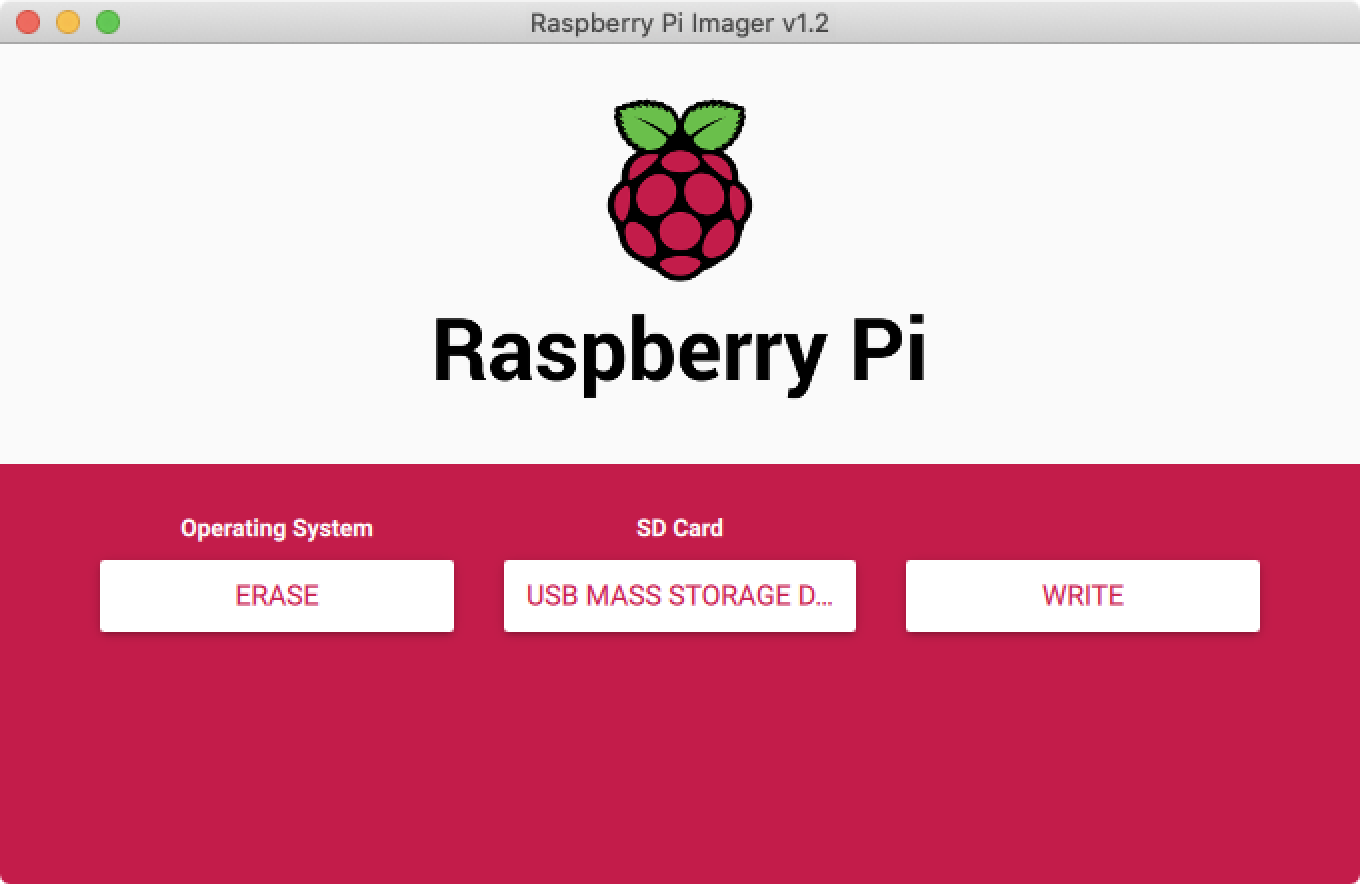
\includegraphics[width=1.0\textwidth]{screenshots/imager-erase.png}
	\caption{Using Raspberry Pi Imager to erase and format a MicroSD card.}
\end{figure}

Then use the Raspberry Pi Imager to write preinstalled server image to the MicroSD card...

\begin{figure}
	\centering	
	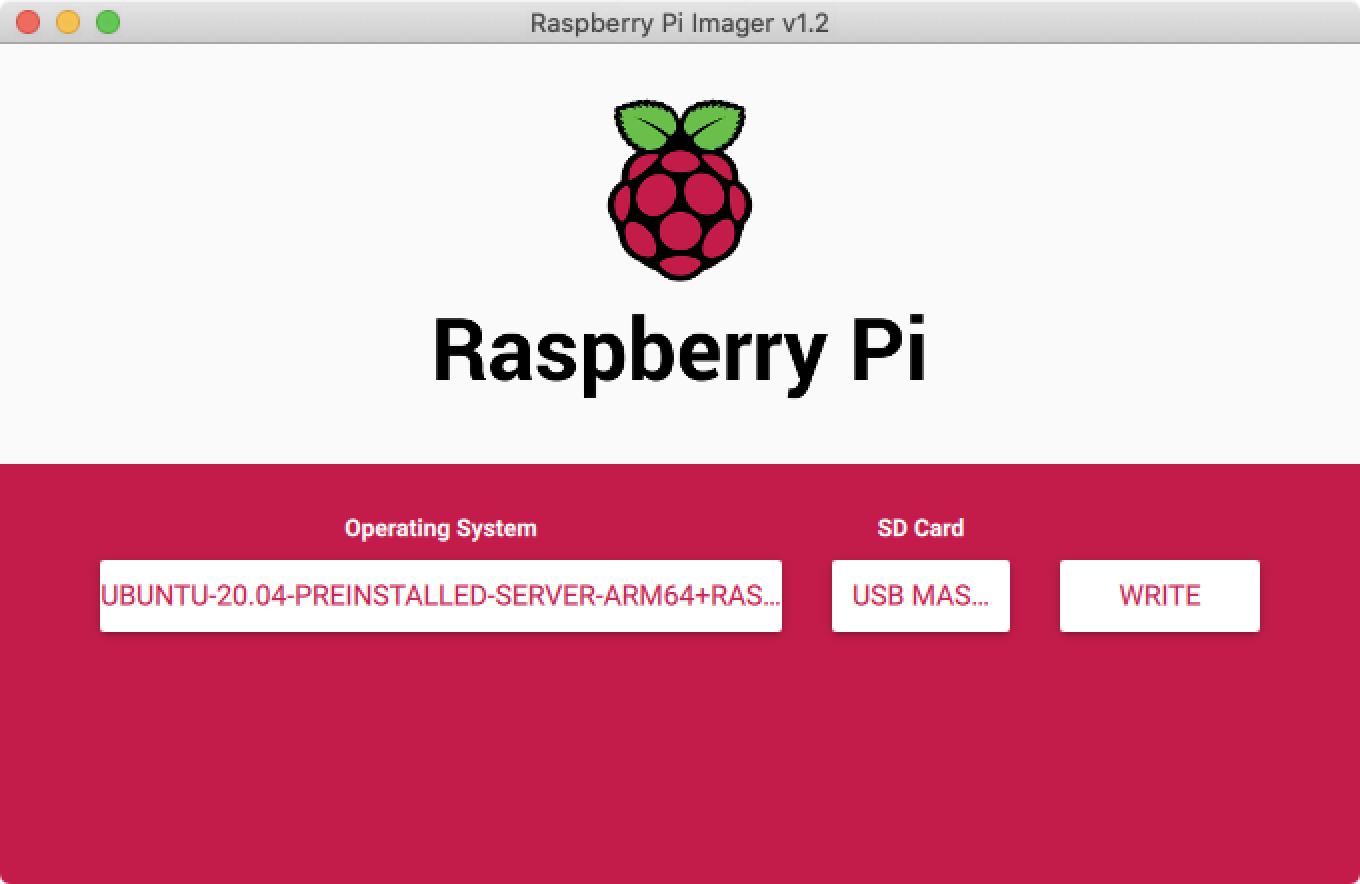
\includegraphics[width=1.0\textwidth]{screenshots/imager-write.png}
	\caption{Using Raspberry Pi Imager to write the server image to a MicroSD card.}
\end{figure}

When complete, remove the MicroSD card from the card reader, place it the Raspberry Pi and plug in the power cable.

The cloud-init configuration process will now start. The Raspberry Pi will acquire its IP address from the router, setup users, update apt, upgrade the system, download software packages, set the hostname (based on the IP address), and finally the system will reboot.


%
% SECTION
%
\clearpage\section{Post-Installation Tasks}

\subsection{Enable No Password Access}

This is required for Open-MPI...

Our public key was installed on each node by cloud-init. So, we can ssh into each node without a password, and use the abbreviated ssh node1, instead of ssh john@node1 (assuming john is the user name on the workstation).

We need to copy our private key to node1 (only node1)...

\lstset{style=termstyle}
\begin{lstlisting}
$ scp ~/.ssh/id_rsa node1:~/.ssh
\end{lstlisting}

Then to enable access to nodes node2 to node9 without a password from node1, we need to import the ... keys into the node1 knownhosts file...

This is easily done. From \verb|macbook|...

\lstset{style=termstyle}
\begin{lstlisting}[]
$ ssh node1
\end{lstlisting}

And then from node1, for \verb|node2| to \verb|node9|...

\lstset{style=termstyle}
\begin{lstlisting}[]
$ ssh node2
\end{lstlisting}

This will generate will generate a message similar to...

\lstset{style=termstyle}
\begin{lstlisting}[]
The authenticity of host 'node2 (192.168.0.2)' can't be established.
ECDSA key fingerprint is SHA256:5VgsnN2nPvpfbJmALh3aJdOeT/NvDXqN8TCreQyNaFA.
Are you sure you want to continue connecting (yes/no/[fingerprint])?
\end{lstlisting}

Respond yes to this, which imports the host key into the \verb|~/.ssh/knownhosts| file of \verb|node1|.

And then exit from the connected node...

\lstset{style=termstyle}
\begin{lstlisting}[]
$ exit
\end{lstlisting}

Repeat the above for \verb|node2| to \verb|node9|.

The above is only required to be done once (unless the host keys on \verb|node2| to \verb|node9| change).


%
% SUB SECTION
%

\subsection{Uninstall unattended-upgrades}

The \verb|unattended-upgrades| package is installed automatically...

This can potentially interferer with long running benchmarks...

Remove...

From \verb|macbook|:

\lstset{style=termstyle}
\begin{lstlisting}[]
$ ssh node1
$ ~/picluster/tools/do "sudo apt remove unattended-upgrades"
\end{lstlisting}

Don't forget to upgrade your cluster regularly at convenient times with...

\lstset{style=termstyle}
\begin{lstlisting}[]
$ ssh node1
$ ~/picluster/tools/upgrade
\end{lstlisting}


\subsection{Add Ubuntu Source Repositories}

We are going to be rebuilding some packages from source...

\lstset{style=termstyle}
\begin{lstlisting}[]
$ ssh node1
$ sudo touch /etc/apt/sources/list.d/picluster.list
$ sudo vim /etc/apt/sources/list.d/picluster.list
\end{lstlisting}

... and add the following source repositories...

\lstset{style=listingstyle}
\begin{lstlisting}[caption=/etc/apt/sources.list.d/picluster.list]
deb-src http://archive.ubuntu.com/ubuntu focal main universe
deb-src http://archive.ubuntu.com/ubuntu focal-updates main universe
\end{lstlisting}

... and then update the repository cache...

\lstset{style=termstyle}
\begin{lstlisting}[]
$ sudo apt update
\end{lstlisting}



\subsection{Create a Project Repository}

Xpand upon...

\lstset{style=termstyle}
\begin{lstlisting}[]
$ ssh node1
$ mkdir picluster
$ cd picluster
$ git init
\end{lstlisting}

Ensure you do push your repository to a remote repository at regular intervals...


\subsection{Select BLAS Library}

The \verb|cloud-init| process will have installed four BLAS libraries, namely...

\verb|libopenblas0-serial|

\verb|libopenblas0-openmp|

\verb|libblis0-serial|

\verb|libblis0-openmp|

To query the BLAS library currently in use on each node we can use one of our Pi Cluster tools...

\lstset{style=termstyle}
\begin{lstlisting}[]
$ ~/picluster/tools/libblas-query
\end{lstlisting}

\lstset{style=termstyle}
\begin{lstlisting}[]
node8... /usr/lib/aarch64-linux-gnu/openblas-openmp/libblas.so.3
node7... /usr/lib/aarch64-linux-gnu/openblas-openmp/libblas.so.3
node6... /usr/lib/aarch64-linux-gnu/openblas-openmp/libblas.so.3
node5... /usr/lib/aarch64-linux-gnu/openblas-openmp/libblas.so.3
node4... /usr/lib/aarch64-linux-gnu/openblas-openmp/libblas.so.3
node3... /usr/lib/aarch64-linux-gnu/openblas-openmp/libblas.so.3
node2... /usr/lib/aarch64-linux-gnu/openblas-openmp/libblas.so.3
node1... /usr/lib/aarch64-linux-gnu/openblas-openmp/libblas.so.3
\end{lstlisting}

To select an alternative library we can use another of our Pi Cluster tools...

\lstset{style=termstyle}
\begin{lstlisting}[]
$ ~/picluster/tools/libblas-set blis-serial
\end{lstlisting}

\lstset{style=termstyle}
\begin{lstlisting}[]
node8... done
node7... done
node6... done 
node5... done 
node4... done 
node3... done 
node2... done 
node1... done 
\end{lstlisting}

\lstset{style=termstyle}
\begin{lstlisting}[]
$ ~/picluster/tools/libblas-query
\end{lstlisting}

\lstset{style=termstyle}
\begin{lstlisting}[]
node8... /usr/lib/aarch64-linux-gnu/blis-serial/libblas.so.3
node7... /usr/lib/aarch64-linux-gnu/blis-serial/libblas.so.3
node6... /usr/lib/aarch64-linux-gnu/blis-serial/libblas.so.3
node5... /usr/lib/aarch64-linux-gnu/blis-serial/libblas.so.3
node4... /usr/lib/aarch64-linux-gnu/blis-serial/libblas.so.3
node3... /usr/lib/aarch64-linux-gnu/blis-serial/libblas.so.3
node2... /usr/lib/aarch64-linux-gnu/blis-serial/libblas.so.3
node1... /usr/lib/aarch64-linux-gnu/blis-serial/libblas.so.3
\end{lstlisting}


%
% SECTION
%
\clearpage\section{Install High-Performance Linpack (HPL)}

Download and install the latest version of HPL on \verb|node1|...

\lstset{style=termstyle}
\begin{lstlisting}
$ ssh node1
$ cd ~/picluster
$ mkdir hpl
$ cd hpl
$ wget https://www.netlib.org/benchmark/hpl/hpl-2.3.tar.gz
$ gunzip hpl-2.3.tar.gz
$ tar xvf hpl-2.3.tar
$ rm hpl-2.3.tar
$ cd hpl-2.3
\end{lstlisting}

Create a \verb|Make.picluster| file...

\lstset{style=termstyle}
\begin{lstlisting}
$ cd setup
$ bash make_generic
$ cp Make.UNKNOWN ../Make.picluster
$ cd ..
\end{lstlisting}

Amend \verb|Make.picluster| as per listing ???.

\lstset{style=listingstyle}
\lstinputlisting[caption=~/picluster/hpl/hpl-2.3/Make.picluster]{picluster/hpl/hpl-2.3/Make.picluster}

Build HPL...

\lstset{style=termstyle}
\begin{lstlisting}
$ make arch=picluster   
\end{lstlisting}

This creates the executable \verb|xhpl| and input file \verb|HPL.dat| in \verb|bin/picluster|

The \verb|xhpl| executable has to exist in the same location on each node, so copy \verb|xhpl| to \verb|node2| to \verb|node8| (only \verb|xhpl|, and not \verb|HPL.dat|)...

\lstset{style=termstyle}
\begin{lstlisting}
$ cd bin/picluster
$ ~/picluster/tools/do "mkdir -p picluster/hpl/hpl-2.3/bin/picluster"
$ scp xhpl node2:~picluster/hpl/hpl-2.3/bin/picluster
$ scp xhpl node3:~picluster/hpl/hpl-2.3/bin/picluster
$ scp xhpl node4:~picluster/hpl/hpl-2.3/bin/picluster
$ scp xhpl node5:~picluster/hpl/hpl-2.3/bin/picluster
$ scp xhpl node6:~picluster/hpl/hpl-2.3/bin/picluster
$ scp xhpl node7:~picluster/hpl/hpl-2.3/bin/picluster
$ scp xhpl node8:~picluster/hpl/hpl-2.3/bin/picluster
\end{lstlisting}



%
% SECTION
%
\clearpage\section{Kernel Build Procedure}

This procedure is derived from the Ubuntu Wiki BuildYourOwnKernel document...

Make sure you have made the source code repositories available as per...

Create a kernel build directory with the correct directory permissions to prevent source download warnings. 

\lstset{style=termstyle}
\begin{lstlisting}
$ ssh node1
$ mkdir -p ~/picluster/build/kernel
$ sudo chown _apt:root ~/picluster/build/kernel
$ cd ~/picluster/build/kernel
\end{lstlisting}

Install the kernel build dependencies...

\lstset{style=termstyle}
\begin{lstlisting}
$ sudo apt-get build-dep linux linux-image-$(uname -r)
\end{lstlisting}

Download the kernel source...

\lstset{style=termstyle}
\begin{lstlisting}
$ sudo apt-get source linux-image-$(uname -r)
$ cd linux-raspi-5.4.0
\end{lstlisting}

This bit is a fix for the subsequent \verb|editconfigs| step of the build procedure...

\lstset{style=termstyle}
\begin{lstlisting}
$ cd debian.raspi/etc
$ sudo cp kernelconfig kernelconfig.original
$ sudo vim kernelconfig
\end{lstlisting}

And make the following change...

\lstset{style=listingstyle}
\begin{lstlisting}[caption=diff kernelconfig kernelconfig.original, numbers=none]
5c5
< 	archs="arm64"
---
> 	archs="armhf arm64"
\end{lstlisting}

Then move back up to the kernel source top level directory...

\lstset{style=termstyle}
\begin{lstlisting}
$ cd ../..
\end{lstlisting}

Prepare the build scripts...

\lstset{style=termstyle}
\begin{lstlisting}
$ sudo chmod a+x debian/rules
$ sudo chmod a+x debian/scripts/*
$ sudo chmod a+x debian/scripts/misc/*
\end{lstlisting}

SOURCE CHANGES AND/OR verb|editconfigs| AT THIS POINT

\lstset{style=termstyle}
\begin{lstlisting}
$ sudo apt install libncurses-dev
$ sudo LANG=C fakeroot debian/rules clean
$ sudo LANG=C fakeroot debian/rules editconfigs
\end{lstlisting}

Tweak the kernel name for identification...

\lstset{style=termstyle}
\begin{lstlisting}
$ cd debian.raspi
$ sudo cp changelog changelog.original
$ sudo vim changelog
\end{lstlisting}

And make the following change, where \verb|+picluster0| is our kernel identifier...

\lstset{style=listingstyle}
\begin{lstlisting}[caption=diff changelog changelog.original, numbers=none]
1c1
< linux-raspi (5.4.0-1015.15+picluster0) focal; urgency=medium
---
> linux-raspi (5.4.0-1015.15) focal; urgency=medium
\end{lstlisting}

Move up to the top level kernel source directory...

\lstset{style=termstyle}
\begin{lstlisting}
$ cd ..
\end{lstlisting}

And build the kernel...

\lstset{style=termstyle}
\begin{lstlisting}
$ sudo LANG=C fakeroot debian/rules clean
$ sudo LANG=C fakeroot debian/rules binary-arch
cd ..
\end{lstlisting}

Install the new kernel...

\lstset{style=termstyle}
\begin{lstlisting}
$ sudo dpkg -i linux*picluster0*.deb
$ sudo shutdown -r now
\end{lstlisting}

Another build procedure fix...

After each kernel build delete the \verb|linux-libc-dev| directory...

\lstset{style=termstyle}
\begin{lstlisting}
$ cd ~/picluster/build/kernel/linux-raspi-5.4.0/debian
$ rm -rf linux-libc-dev
$ cd ..
\end{lstlisting}


%
% SECTION
%
\clearpage\section{Build Kernel with Jumbo Frames Support}

Standard MTU is 1500 bytes...

Maximum payload size is 1472 bytes...

NB of 184 (x 8 bytes for Double Precision) = 1472 bytes...

NB $>$ 184 $=>$ packet fragmentation $=>$ reduced network efficiency...

This causes drop of in performance???...

Max MTU on Raspberry Pi 4 Model B is set at build time to 1500...

Not configurable above 1500...

TODO: EXAMPLE OF ERROR MSG...

Need to build the kernel with higher MTU...


Make the required changes to the source... as per REFERENCE

\begin{verbatim}
    cd linux-raspi-5.4.0 

    sudo vim include/linux/if_vlan.h...
        #define VLAN_ETH_DATA_LEN   9000
        #define VLAN_ETH_FRAME_LEN  9018
    
    sudo vim include/uapi/linux/if_ether.h...
        #define ETH_DATA_LEN        9000
        #define ETH_FRAME_LEN       9014
    
    sudo vim drivers/net/ethernet/broadcom/genet/bcmgenet.c...
        #define RX_BUF_LENGTH       10240
\end{verbatim}

Add a Jumbo Frames identifier, "+jf", to the new kernel name...

\begin{verbatim}
    sudo vim debian.raspi/changelog...
        linux (5.4.0-1013.13+jf) focal; urgency=medium
        
\end{verbatim}



%
% SECTION
%
\clearpage\section{Rebuild OpenBLAS}

\lstset{style=termstyle}
\begin{lstlisting}
$ ssh node1
$ mkdir -p build/openblas
$ chown -R _apt:root build
$ cd build/openblas
$ sudo apt-get source openblas
$ sudo apt-get build-dep openblas
$ cd openblas-0.3.8+ds
\end{lstlisting}


Edit cpuid\_arm64.c...

\lstset{style=termstyle}
\begin{lstlisting}
$ sudo cp cpuid_arm64.c cpuid_arm64.c.original
$ sudo vim cpuid_arm64.c
\end{lstlisting}


\lstset{style=termstyle}
\begin{lstlisting}
$ diff cpuid_arm64.c cpuid_arm64.c.original
\end{lstlisting}

\lstset{style=termstyle}
\begin{lstlisting}
275c275
<       printf("#define L2_SIZE 1048576\n");
---
>       printf("#define L2_SIZE 524288\n");
278c278
<       printf("#define DTB_DEFAULT_ENTRIES 32\n");
---
>       printf("#define DTB_DEFAULT_ENTRIES 64\n");
\end{lstlisting}


And, then following the instructions in debian/README.Debian

\lstset{style=termstyle}
\begin{lstlisting}
$ DEB_BUILD_OPTIONS=custom dpkg-buildpackage -uc -b
\end{lstlisting}

Once the build is complete..

\lstset{style=termstyle}
\begin{lstlisting}
cd ..
$ sudo apt remove libopenblas0-serial
$ sudo dpkg -i libopenblas0-serial\_0.3.8+ds-1\_arm64.deb
\end{lstlisting}

Ensure the correct BLAS library is being used...

\lstset{style=termstyle}
\begin{lstlisting}
$ sudo update-alternatives --config libblas.so.3-aarch64-linux-gnu
\end{lstlisting}

copy to other nodes
remove old...
install new...

If more than one BLAS library is installed, check update-alternatives!!!

ssh node2 .. node8
\lstset{style=termstyle}
\begin{lstlisting}
$ ssh node2 sudo apt remove libblas0-serial
$ scp libopenblas0-serial\_0.3.8+ds-1\_arm64.deb node2:~
$ ssh sudo dpkg -i libopenblas0-serial\_0.3.8+ds-1\_arm64.deb
$ ssh sudo update-alternatives --config libblas.so.3-aarch64-linux-gnu
\end{lstlisting}


%
% SECTION
%
\clearpage\section{Rebuild BLIS}

\lstset{style=termstyle}
\begin{lstlisting}
$ ssh node1
$ mkdir -p picluster/build/blis
$ cd picluster/build/blis
$ apt-get source blis
$ sudo apt-get build-dep blis
$ cd blis-0.6.1
\end{lstlisting}



%
% SECTION
%
\clearpage\section{Pi Cluster Tools}

\lstinputlisting[caption=picluster/tools/upgrade, numbers=left, backgroundcolor=\color{LightSkyBlue}]{picluster/tools/upgrade}
\lstinputlisting[caption=picluster/tools/reboot, numbers=left, backgroundcolor=\color{LightSkyBlue}]{picluster/tools/reboot}
\lstinputlisting[caption=picluster/tools/shutdown, numbers=left, backgroundcolor=\color{LightSkyBlue}]{picluster/tools/shutdown}
\lstinputlisting[caption=picluster/tools/libblas-query, numbers=left, backgroundcolor=\color{LightSkyBlue}]{picluster/tools/libblas-query}
\lstinputlisting[caption=picluster/tools/libblas-set, numbers=left, backgroundcolor=\color{LightSkyBlue}]{picluster/tools/libblas-set}



%
% SECTION
%

\clearpage\section{Build OpenMPI from Source}

Do all of this on node1...

\lstset{style=termstyle}
\begin{lstlisting}
$ ssh node1
\end{lstlisting}

We want to avoid collisions with multiple OpenMPI installations, so remove original installed version...

\lstset{style=termstyle}
\begin{lstlisting}
$ sudo apt remove openmpi-common
$ sudo apt remove openmpi-bin
$ sudo apt autoremove 
\end{lstlisting}

OpenMPI requires the libevent-dev package...

\lstset{style=termstyle}
\begin{lstlisting}
$ sudo apt install libevent-dev
\end{lstlisting}

Create a build directory, and download and, and and following BLAH, BLAH build OpenMPI...

\lstset{style=termstyle}
\begin{lstlisting}
$ mkdir -p ~/picluster/build/openmpi
$ cd ~/picluster/build/openmpi
$ wget https://download.open-mpi.org/release/open-mpi/v4.0/openmpi-4.0.4.tar.gz
$ gunzip openmpi-4.0.4.tar.gz
$ tar xvf openmpi-4.0.4.tar
$ rm openmpi-4.0.4.tar
$ cd openmpi-4.0.4
$ mkdir build
$ cd build
$ ../configure CFLAGS="-O3 -march=armv8-a -mtune=cortex=a72"
$ make all
$ sudo make install
$ sudo ldconfig
\end{lstlisting}

OpenMPI will installed to /usr/local

EXTRACT FROM HPL.dat


TODO: HOW TO COPY TO ALL NODES!



%
% SECTION
%

\clearpage\section{Arm Performance Libraries}

\textcolor{red}{This does not work yet! HPL will build, but raises an illegal instruction error at runtime. At the time of writing, Arm Performance Libraries release 20.2.0 require a minimum of armv8.1-a. Unfortunately, the Raspberry Pi's Cortex-A72 cores are armv8.0-a. The next release will support armv8.0-a. Appendix included for future reference.}  

"Arm Performance Libraries provides optimized standard core math libraries for high-performance computing applications on Arm processors. This free version of the libraries provides optimized libraries for Arm® Neoverse™ N1-based Armv8 AArch64 implementations that are compatible with various versions of GCC. You do not require a license for this version of the libraries."

Downloaded Arm Performance Libraries 20.2.0 with GCC 9.3 for Ubuntu 16.04+.

\lstset{style=termstyle}
\begin{lstlisting}
$ ssh node1
$ sudo apt install environment-modules
$ mkdir picluster/armpl
$ cd picluster/armpl
$ tar xvf arm-performance-libraries_20.2_Ubuntu-16.04_gcc-9.3.tar
$ rm arm-performance-libraries_20.2_Ubuntu-16.04_gcc-9.3.tar
$ sudo ./arm-performance-libraries_20.2_Ubuntu-16.04.sh
\end{lstlisting}

The default installation directory is /opt/arm...

TODO: CHANGE TO /usr/local + ldconfig

Compile HPL with armpl...

\lstset{style=termstyle}
\begin{lstlisting}
$ cd ~/picluster/hpl/hpl-2.3
$ cp Make.serial Make.armpl-serial
\end{lstlisting}

Edit Make.armpl-serial...

\lstset{style=listingstyle}
\begin{lstlisting}[caption=Make.armpl-serial extract]
# ----------------------------------------------------------------------
# - Linear Algebra library (BLAS or VSIPL) -----------------------------
# ----------------------------------------------------------------------
# LAinc tells the  C  compiler where to find the Linear Algebra  library
# header files,  LAlib  is defined  to be the name of  the library to be 
# used. The variable LAdir is only used for defining LAinc and LAlib.
#
LAdir        = /opt/arm/armpl_20.2_gcc-9.3
LAinc        =
LAlib        = -L$(LAdir)/lib -larmpl -lgfortran -lamath -lm
\end{lstlisting}

Compile HPL...

\lstset{style=termstyle}
\begin{lstlisting}[]
$ make arch=armpl-serial
\end{lstlisting}



%
% THE END
%
\end{document}
